% !TEX root = task-2-10-7.tex
% Editable task bank. Append new BankTask blocks at the end of the document.
\documentclass[12pt,a4paper]{article}
\usepackage{physics-textbook}
\usepackage{graphicx,needspace}
\usetikzlibrary{decorations.pathmorphing}
\newif\ifShowSolutions
\ifdefined\TutorEdition
  \ShowSolutionstrue
\else
  \ShowSolutionsfalse % Change to \ShowSolutionstrue to display solutions.
\fi
\newcounter{banktask}
\newsavebox{\BankTaskBox}
\newcommand{\BankTaskContent}[3]{%
  \noindent\textbf{\thebanktask.}\quad #2\par
  \ifShowSolutions
    \Needspace{50mm}% Keep the solution heading with its opening text or diagram.
    #3\par
    \ifdefined\TutorEdition
      \ifcsname TutorSource#1\endcsname
        \nopagebreak\smallskip{\small\csname TutorSource#1\endcsname\par}%
      \fi
    \fi
  \fi
}
\newcommand{\BankTask}[3]{%
  \refstepcounter{banktask}\par\medskip
  \sbox{\BankTaskBox}{\begin{minipage}{\linewidth}%
    \BankTaskContent{#1}{#2}{#3}\end{minipage}}%
  \ifdim\dimexpr\ht\BankTaskBox+\dp\BankTaskBox\relax>\dimexpr\textheight-20mm\relax
    \Needspace{35mm}\BankTaskContent{#1}{#2}{#3}%
  \else
    \Needspace{\dimexpr\ht\BankTaskBox+\dp\BankTaskBox\relax}%
    \noindent\usebox{\BankTaskBox}\par
  \fi
  \medskip
}
\begin{document}
\BookSubsection{2.10.7}{График кипения}


% Source 217002: https://ege.fipi.ru/bank/questions.php?search=1&proj=BA1F39653304A5B041B656915DC36B38&qid=217002
\BankTask{217002}{
\begin{center}
\begin{tikzpicture}[task graph,x=1.5cm,y=1cm]
\draw[task axis] (0,0)--(3.8,0) node[below] {$Q,\,10^4\,\text{Дж}$};
\draw[task axis] (0,0)--(0,3) node[left] {$t,\,{}^\circ\text{C}$};
\node[below left] at (0,0) {$0$};
\foreach \x in {0.5,1,1.5,2} {
\draw[task projection] (\x,0)--(\x,1.75);
}
\draw[task projection] (2.55,0)--(2.55,2.50625);
\draw[task curve] (0,0.8)--(0.5,1.75)--(2,1.75)--(2.8,2.85);
\node[below] at (1,0) {$1$};
\node[below] at (2,0) {$2$};
\end{tikzpicture}
\end{center}
На рисунке показан график изменения температуры вещества по мере поглощения им количества теплоты. Вещество находится в сосуде под поршнем. Масса вещества равна $0{,}5\,\text{кг}$. Первоначально вещество было в жидком состоянии. Какова удельная теплота парообразования вещества (в $\text{кДж}/\text{кг}$)?
}{
\smallskip\noindent\textbf{Решение от GPT}\par
Горизонтальный участок соответствует парообразованию. На него затрачено
\[
Q_{\text{пар}}=(2-0{,}5)\cdot10^4=1{,}5\cdot10^4\,\text{Дж}.
\]
Удельная теплота парообразования
\[
L=\frac{Q_{\text{пар}}}{m}=\frac{1{,}5\cdot10^4}{0{,}5}=3\cdot10^4\,\text{Дж}/\text{кг}=30\,\text{кДж}/\text{кг}.
\]
Ответ: $30$.
}

% Source F72E75: https://ege.fipi.ru/bank/questions.php?search=1&proj=BA1F39653304A5B041B656915DC36B38&qid=F72E75
\BankTask{F72E75}{
На рисунке представлены графики зависимости температуры \(t\) двух тел одинаковой массой от сообщённого им количества теплоты \(Q\). Каждое тело находится в сосуде под поршнем. Первоначально тела находились в жидком агрегатном состоянии.
\begin{center}
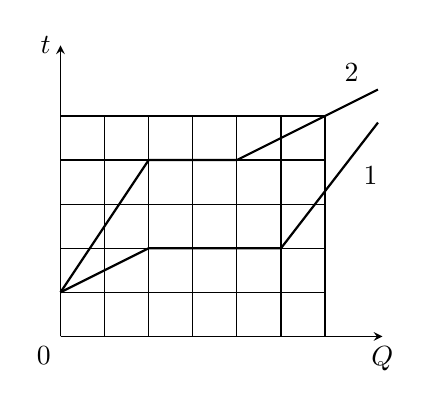
\begin{tikzpicture}[>=stealth,x=0.56cm,y=0.56cm]
\draw[step=1,thin] (0,0) grid (6,5);
\draw[->] (0,0)--(7.3,0) node[below] {$Q$};
\draw[->] (0,0)--(0,6.6) node[left] {$t$};
\node[below left] at (0,0) {$0$};
\draw[thick] (0,1)--(2,2)--(5,2)--(7.2,4.85);
\draw[thick] (0,1)--(2,4)--(4,4)--(7.2,5.6);
\node[right] at (6.65,3.65) {$1$};
\node[above] at (6.6,5.55) {$2$};
\end{tikzpicture}
\end{center}
\begin{enumerate}
\item Температура кипения первого тела в \(2\) раза меньше, чем температура кипения второго тела.
\item Тела имеют одинаковую удельную теплоёмкость в газообразном состоянии.
\item Удельная теплоёмкость в жидком агрегатном состоянии у второго тела в \(3\) раза меньше, чем у первого.
\item Оба тела имеют одинаковую удельную теплоту парообразования.
\item Для первого тела удельная теплоёмкость в жидком агрегатном состоянии меньше удельной теплоёмкости в газообразном состоянии.
\end{enumerate}
}{
\smallskip\noindent\textbf{Решение от GPT}\par
При нагревании \(c=\Delta Q/(m\Delta t)\), при кипении \(L=\Delta Q/m\). Массы одинаковы.
\begin{enumerate}
\item Верно: горизонтальные участки расположены на уровнях \(2\) и \(4\) клеток от нуля температуры, поэтому \(t_{\text{кип},1}=t_{\text{кип},2}/2\).
\item Неверно: наклоны участков нагревания пара различаются, следовательно, теплоёмкости различны.
\item Верно: при одинаковом количестве теплоты на начальных участках \(\Delta t_1=1\) клетка, \(\Delta t_2=3\) клетки. Поэтому \(c_2=c_1/3\).
\item Неверно: длины участков кипения равны \(3\) и \(2\) клеткам по оси \(Q\), поэтому \(L_1/L_2=3/2\).
\item Неверно: участок нагревания пара первого тела круче участка нагревания жидкости, поэтому \(c_{\text{газ},1}<c_{\text{ж},1}\).
\end{enumerate}
\(\boxed{13}\).
}

% Source E2B7DC: https://ege.fipi.ru/bank/questions.php?search=1&proj=BA1F39653304A5B041B656915DC36B38&qid=E2B7DC
\BankTask{E2B7DC}{
В начальный момент в сосуде под лёгким поршнем находится только жидкий эфир. На рисунке схематично представлен график зависимости температуры \(t\) эфира от времени \(\tau\) его нагревания и последующего охлаждения.
\begin{center}
\begin{tikzpicture}[x=0.85cm,y=0.65cm,>=stealth]
\draw[->] (0,0)--(6.8,0) node[below] {$\tau$};
\draw[->] (0,0)--(0,4.7) node[left] {$t,\,{}^\circ\mathrm{C}$};
\node[below left] at (0,0) {$0$};
\foreach \y/\v in {1/20,2/40,3/60}{\draw (-0.08,\y)--(0.08,\y);\node[left] at (-0.1,\y) {$\v$};}
\foreach \y in {0.5,1.5,2.5}{\draw (-0.06,\y)--(0.06,\y);}
\draw[dashed] (0,2)--(3.35,2);
\draw (0,1)--(0.75,2)--(2.1,2)--(2.72,3.4)--(3.35,2)--(4.7,2)--(5.35,1);
\node[below right] at (0,1) {$A$};
\node[above] at (0.75,2) {$B$};
\node[above left] at (2.1,2) {$C$};
\node[above] at (2.72,3.4) {$D$};
\node[above right] at (3.35,2) {$E$};
\node[above right] at (4.7,2) {$F$};
\node[right] at (5.35,1) {$G$};
\end{tikzpicture}
\end{center}
\begin{enumerate}
\item Температура кипения эфира равна \(60\,{}^\circ\mathrm{C}\).
\item В точке \(F\) в сосуде находился только жидкий эфир.
\item На участке \(BC\) внутренняя энергия эфира увеличивалась.
\item В точке \(G\) эфир отвердел.
\item Время, за которое весь эфир выкипел, меньше, чем время, за которое он сконденсировался.
\end{enumerate}
}{
\smallskip\noindent\textbf{Решение от GPT}\par
1) Неверно: горизонтальный участок $BC$ соответствует кипению при $40\,{}^\circ\text{C}$.

2) Верно: в точке $F$ конденсация завершилась, далее охлаждается жидкость.

3) Верно: при кипении внутренняя энергия увеличивается за счёт увеличения потенциальной энергии взаимодействия молекул.

4) Неверно: участок $FG$ соответствует охлаждению жидкости; признаков отвердевания нет.

5) Неверно: участки $BC$ и $EF$ на схематическом графике имеют одинаковую длительность.

Ответ: $23$.
}

\end{document}
